
\section{Introduction}


\begin{frame}
\frametitle{Overview}  

\begin{itemize}[<+->]
  \item The B method supports the construction of safety systems
  \begin{itemize}
    \item Until the implementation model
    \item But the result of this translation is not guaranteed by formal means
    \item Then the transformation process can introduce small bugs\\
       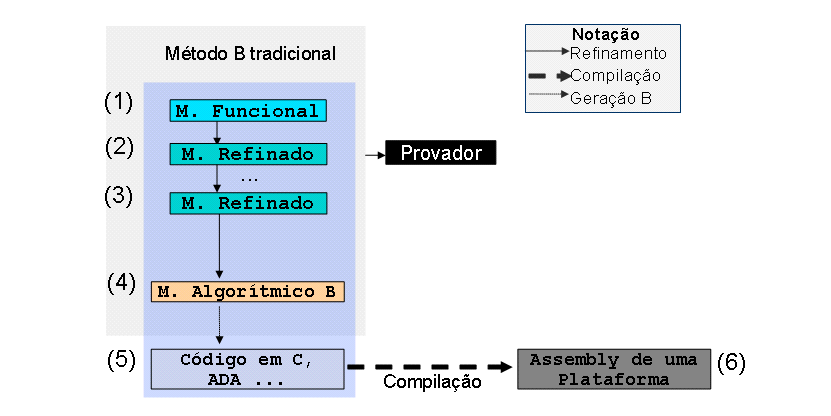
\includegraphics[width=.7\textwidth]{figures/passos_de_desenvolvimento_tradicional.png}
  \end{itemize}
  \item The last year a paper [Dantas, 2008] proposed a approach to extend the formal verification
  \item One key of this approach is the formal model of the instruction set  of execution platform % of such assembly languages
\end{itemize}
% TO-DO Ajustar a figura   

	\note{ ................... }
\end{frame}



\begin{frame}
\frametitle{Overview}  

\begin{itemize}[<+->]
  \item The B method supports the construction of safety systems
  \begin{itemize}
    \item Until the implementation model
    \item But the result of this translation is not guaranteed by formal means
    \item Then the transformation process can introduce small bugs\\
       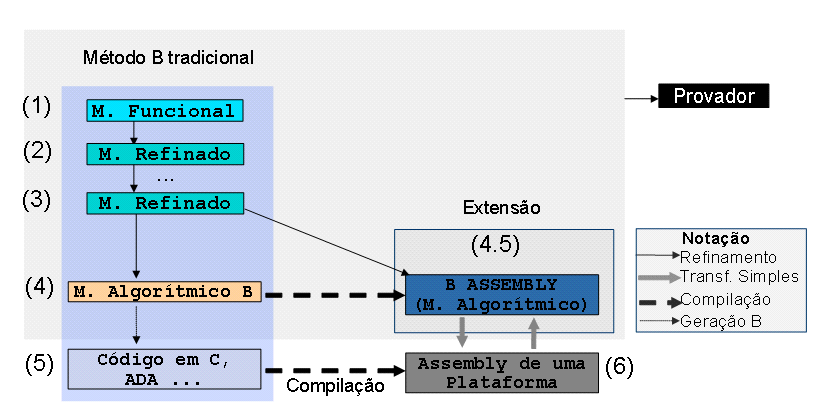
\includegraphics[width=.7\textwidth]{figures/passos_de_desenvolvimento_extendido.png}
  \end{itemize}
  \item The last year a paper [Dantas, 2008] proposed a approach to extend the formal verification
  \item One key of this approach is the formal model of the instruction set  of execution platform % of such assembly languages
\end{itemize}
% TO-DO Ajustar a figura

	\note{ ................... }
\end{frame}


\begin{frame}
\frametitle{Modelling}  

\begin{itemize}[<+->]
  \item The modelling is builded using some libraries developed
  \item The libraries has common concepts that can be used to others platforms too
  \item Utilities of this Formal Model:
  \begin{itemize}
    \item Documentation
    \item Simulation
    \item The formal verification until the assembly level
    \item A possible support to verify the Z80 design

  \end{itemize}
\end{itemize}

	\note{ ................... }
\end{frame}



\begin{frame}
\frametitle{Objective}  

\begin{itemize}[<+->]
  \item The main actual objective is represent the instruction set
    \begin{itemize}
    \item The aspects no-functional are not represented: logic circuits, pipeline, data bus, \ldots 
  \end{itemize}
  \item Because there are many efficient ways to verify hardware

\end{itemize}
% 

	\note{ ................... }
\end{frame}



